% =====================================================================
%  CSRS -- Internship Work Record
%  Build:  ./latex/build.sh          (tectonic, XeTeX)
%  Figures: latex/make_figures.py    -- data figures from eval/final/summary.csv
%           latex/make_excerpts.py   -- deliverable cards from the alert artefacts
%           latex/make_screenshots.sh -- live UI captures
%  Everything below is content; the style block is the first section.
% =====================================================================
\documentclass[11pt,a4paper]{article}

% ---------- fonts (XeTeX / tectonic) ---------------------------------
\usepackage{fontspec}
\usepackage[default,scale=0.96]{sourcesanspro}
\usepackage{sourcecodepro}
\usepackage{microtype}

% ---------- page ------------------------------------------------------
\usepackage[a4paper,top=22mm,bottom=20mm,left=20mm,right=20mm,headsep=7mm,footskip=10mm]{geometry}
\usepackage{xcolor}
\usepackage{graphicx}
\usepackage{float}
\usepackage{booktabs}
\usepackage{tabularx}
\usepackage{ltablex}
\keepXColumns
\usepackage{array}
\usepackage{enumitem}
\usepackage{fancyhdr}
\usepackage{titlesec}
\usepackage[skip=6pt,font={small},labelfont={bf,color=accent}]{caption}
\usepackage[most]{tcolorbox}
\usepackage[hidelinks]{hyperref}

% ---------- palette ---------------------------------------------------
\definecolor{accent}{HTML}{184F95}
\definecolor{accenttint}{HTML}{E8EFF8}
\definecolor{ink}{HTML}{1A1A18}
\definecolor{soft}{HTML}{55544F}
\definecolor{rulegrey}{HTML}{D8D7D2}
\definecolor{surface}{HTML}{FBFBFA}
\color{ink}

% ---------- headings: solid accent band -------------------------------
\renewcommand{\section}[1]{%
  \par\addvspace{16pt}%
  \refstepcounter{section}%
  \addcontentsline{toc}{section}{\thesection\quad #1}%
  \noindent\colorbox{accent}{%
    \begin{minipage}{\dimexpr\textwidth-2\fboxsep\relax}
      \vspace{2.5pt}
      \color{white}\bfseries\large
      \makebox[9mm][l]{\thesection}#1
      \vspace{2.5pt}
    \end{minipage}}%
  \par\nobreak\vspace{9pt}%
}

\titleformat{\subsection}[block]{\normalfont\bfseries\normalsize\color{accent}}{}{0pt}{}
\titlespacing*{\subsection}{0pt}{12pt}{4pt}

% ---------- running head ----------------------------------------------
\pagestyle{fancy}
\fancyhf{}
\renewcommand{\headrulewidth}{0.4pt}
\renewcommand{\headrule}{\color{rulegrey}\hrule height 0.4pt}
\fancyhead[L]{\footnotesize\color{soft}CSRS --- Work Record}
\fancyhead[R]{\footnotesize\color{soft}Muhammad Subhan Amir \quad\textbar\quad\ Information Technology University}
\fancyfoot[C]{\footnotesize\color{soft}\thepage}

% ---------- float placement: let figures share a page -----------------
\renewcommand{\topfraction}{0.92}
\renewcommand{\bottomfraction}{0.92}
\renewcommand{\textfraction}{0.06}
\renewcommand{\floatpagefraction}{0.75}
\setcounter{topnumber}{3}
\setcounter{bottomnumber}{2}
\setcounter{totalnumber}{4}
\raggedbottom

% ---------- helpers ---------------------------------------------------
\setlength{\parindent}{0pt}
\setlength{\parskip}{6pt}
\renewcommand{\arraystretch}{1.25}
\newcolumntype{R}{>{\raggedleft\arraybackslash}X}
\newcolumntype{L}{>{\raggedright\arraybackslash}X}
\newcommand{\code}[1]{{\small\ttfamily #1}}

% A figure wrapped in a light "proof" frame with its caption underneath.
\newenvironment{proofbox}{%
  \begin{tcolorbox}[colback=surface,colframe=rulegrey,boxrule=0.6pt,
    arc=2.5pt,left=5pt,right=5pt,top=6pt,bottom=6pt,enhanced]%
  \centering
}{%
  \end{tcolorbox}
}

\newcommand{\statcell}[2]{%
  \begin{minipage}[t]{0.19\textwidth}
    \centering
    {\color{accent}\bfseries\Large #1}\\[1pt]
    {\footnotesize\color{soft} #2}
  \end{minipage}%
}

\begin{document}

% =====================================================================
% TITLE PAGE
% =====================================================================
\thispagestyle{empty}
\begin{tikzpicture}[remember picture, overlay]
  \fill[accent] (current page.north west) rectangle
    ([yshift=-95mm]current page.north east);
  \node[anchor=north west, text width=150mm, inner sep=0pt, align=left]
    at ([shift={(20mm,-30mm)}]current page.north west) {%
      \color{white}
      {\footnotesize CYBERSECURITY STANDARDS RAG SYSTEM}\\[6mm]
      {\fontsize{34}{40}\selectfont\bfseries CSRS --- Work Record}\\[5mm]
      {\large A local retrieval-augmented generation system for cybersecurity
       standards, and the alert-severity ranking experiment built on it.}%
    };
\end{tikzpicture}

\vspace*{85mm}

\begin{tabularx}{\textwidth}{@{}l X@{}}
  {\color{soft}\small Student}     & \textbf{Muhammad Subhan Amir} \\
  {\color{soft}\small Student ID}  & BSCS23016 \\
  {\color{soft}\small Institution} & Information Technology University \\
  {\color{soft}\small Period}      & 21 July --- 21 August 2026 \\
  {\color{soft}\small Repository}  & \href{https://github.com/subhan-17h/CSRS}{github.com/subhan-17h/CSRS} \\
\end{tabularx}

\vspace{16mm}

\noindent\textcolor{rulegrey}{\rule{\textwidth}{0.6pt}}

\vspace{6mm}

\noindent
\statcell{117}{commits}\hfill
\statcell{16}{working days}\hfill
\statcell{4{,}020}{documents indexed}\hfill
\statcell{343}{automated tests}\hfill
\statcell{5}{models benchmarked}

\vspace{6mm}

\noindent\textcolor{rulegrey}{\rule{\textwidth}{0.6pt}}

\vfill

{\footnotesize\color{soft}
Every figure in this record was produced from the system itself: live screenshots of
the running interfaces, charts computed from the committed evaluation results, and
excerpts regenerated from the experiment's own output files.
\par}

\clearpage

% =====================================================================
\section{What was built}

CSRS answers questions about cybersecurity standards from the standards themselves.
A user asks a question in plain English; the system finds the passages that actually
address it and has a language model write an answer grounded in those passages, with
the source page and section shown alongside. If the corpus does not contain an answer,
it says so rather than inventing one.

The whole pipeline runs on the local machine --- parsing, embedding, search and
generation. No document content leaves the host during normal operation.

\begin{description}[leftmargin=0pt,style=nextline,itemsep=3pt]
  \item[Ingestion] PDFs are parsed by Docling with page boundaries preserved, split
    into roughly 400-token chunks that carry their heading trail and control
    identifier, and embedded locally. Files are fingerprinted by content hash, so
    re-indexing an unchanged corpus does no work.
  \item[Retrieval] A dense vector search over Chroma and a persisted BM25 keyword
    index run in parallel and are combined by reciprocal-rank fusion. Hybrid retrieval
    is the default; an optional reranking stage ships disabled.
  \item[Generation] The top passages are sent to a local Ollama model with a grounding
    instruction. The answer is returned with citations to the retrieved pages.
  \item[Interfaces] A Streamlit application covers the required local UI. A FastAPI
    service plus a React front end add token streaming, source cards, settings, saved
    conversations, a corpus browser and an in-app document viewer.
  \item[Evaluation] A 50-question benchmark scores five local models on three
    independent metrics. A later experiment reuses the same retriever to rank the
    severity of 50 real intrusion-detection alerts.
\end{description}

\begin{figure}[H]
  \centering
  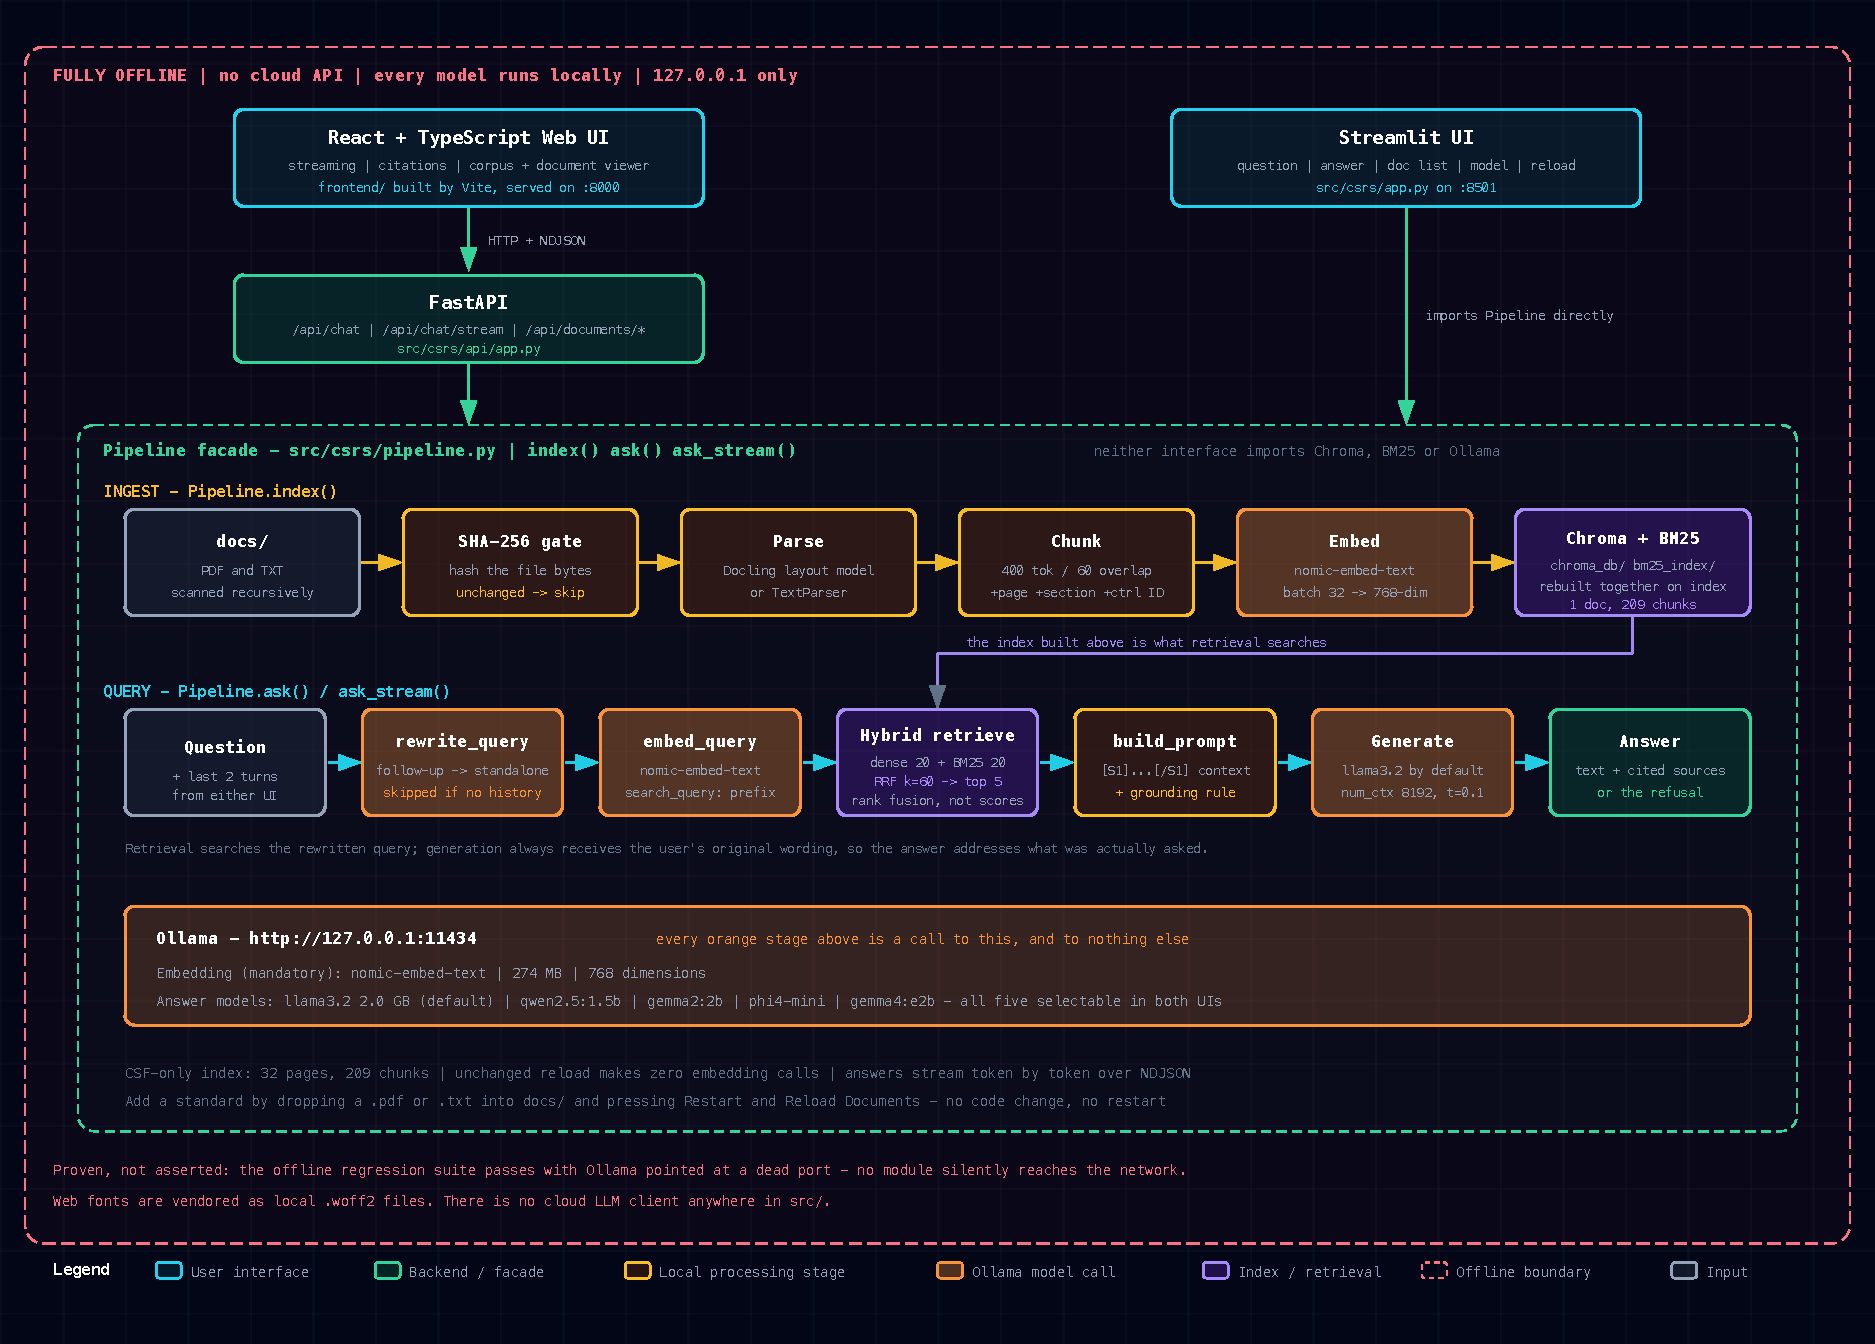
\includegraphics[width=\textwidth]{figures/architecture.pdf}
  \caption{The shipped pipeline. Ingestion on the left of the query path, hybrid
  retrieval in the middle, grounded generation on the right; everything inside the
  dashed boundary runs locally.}
\end{figure}

% =====================================================================
\section{Day-by-day record}

The internship ran from Tuesday 21 July to Friday 21 August 2026. The 32-day span
contains \textbf{16 working days}, on each of which either commits were made or a dated
artefact was produced. Of the remaining dates, seven are weekends and nine are weekdays
spent on background reading and result analysis rather than on committed work.

\begin{figure}[H]
  \centering
  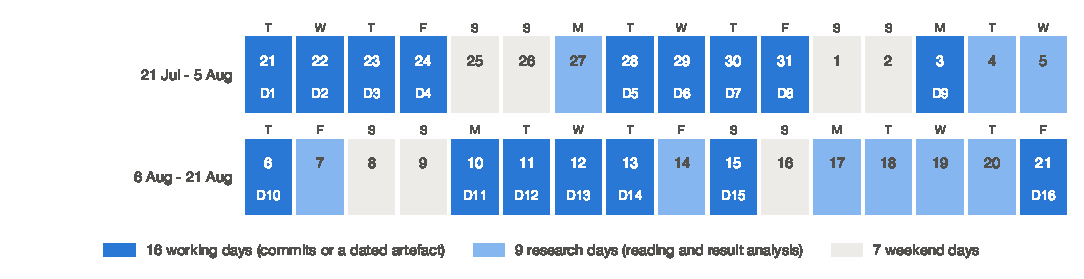
\includegraphics[width=\textwidth]{figures/calendar.pdf}
  \caption{The whole internship at a glance. Dark cells are working days and carry
  their day number; mid cells are research days; pale cells are weekends.}
\end{figure}

Three of the sixteen working days produced no commit, because the work was data
preparation carried out outside the repository. Each is evidenced by the file it wrote,
and each was a precondition for the code that followed.

\subsection{Week 1 --- building the system (21--24 July)}

{\small
\begin{tabularx}{\textwidth}{@{}p{15mm} p{11mm} L@{}}
\toprule
\textbf{Day} & \textbf{Date} & \textbf{Work and result} \\
\midrule
\endhead
Day 1 & 21 Jul & Specification, roadmap, typed configuration, then the first
  end-to-end path: loaders, chunking, prefixed embeddings, vector storage, grounded
  generation, a pipeline facade and a minimal Streamlit UI. Page-aware PDF parsing
  closed the day. \emph{23 commits, +10{,}212/--1{,}101.} \\
Day 2 & 22 Jul & Docling replaced the hand-written PDF heuristics; content-hash
  indexing made re-runs cheap; model warming made offline operation a setup step. The
  Streamlit UI was completed and the FastAPI service and React front end begun.
  \emph{18 commits, +10{,}629/--426.} \\
Day 3 & 23 Jul & Token streaming, settings, the corpus explorer and saved
  conversations. Both interfaces documented and visually verified; corrupt-history
  handling fixed; the first 48-question retrieval golden set added.
  \emph{11 commits, +3{,}399/--255.} \\
Day 4 & 24 Jul & Retrieval measurement, persisted BM25, reciprocal-rank fusion and
  optional reranking. The original target was found to reward duplicate passages from
  one control, so the metric was re-baselined on rank-one relevance and hybrid
  retrieval became the default. Conversational rewriting, document viewing and
  licensing followed. \emph{22 commits, +5{,}380/--796.} \\
\bottomrule
\end{tabularx}
}

\subsection{Week 2 --- measuring it, and turning to alerts (27--31 July)}

{\small
\begin{tabularx}{\textwidth}{@{}p{15mm} p{11mm} L@{}}
\toprule
\textbf{Day} & \textbf{Date} & \textbf{Work and result} \\
\midrule
\endhead
--- & 27 Jul & \emph{Research day.} Reading on how retrieval quality is measured and
  improved, before committing to an evaluation design. \code{RESEARCH.md} records the
  ground covered: fusion and reranking, the finding that Ollama exposes no reranking
  endpoint, and the advanced architectures evaluated and declined --- HyDE, multi-query
  expansion, step-back prompting, late chunking and CRAG --- each with the reason it did
  not suit a local, CPU-bound system. \\
Day 5 & 28 Jul & The retrieval-only harness was replaced by an answer-quality
  evaluation: 20 questions over four documents, cosine similarity, evidence coverage
  and an optional structured judge. \emph{1 commit, +4{,}177/--1{,}856.} \\
Day 6 & 29 Jul & The corpus was reduced to NIST CSF 2.0 and 50 new evidence-grounded
  questions written. All five installed models were compared on three independent
  metrics, producing a complete 250-row result set with no technical errors. The first
  verified work record was written the same day.
  \emph{13 commits, +5{,}218/--3{,}279.} \\
Day 7 & 30 Jul & \emph{No commit; evidenced by its artefact.} The intrusion-alert
  dataset was prepared as \code{enriched\_snort\_alerts.json} (2.7\,MB). The alert
  corpus had to exist before a ranking task could be defined over it. \\
Day 8 & 31 Jul & \emph{No commit; evidenced by its artefacts.} Snort rule
  documentation was collected from snort.org in a scripted browser session, leaving 16
  artefacts: three console logs, nine page snapshots and four screenshots. This
  established which fields the published documentation carries --- category, alert
  message, explanation, properties, CVE and references --- the fields Day 16 would
  render into the corpus. \\
\bottomrule
\end{tabularx}
}

\subsection{Week 3 --- defining severity and ranking alerts (3--7 August)}

{\small
\begin{tabularx}{\textwidth}{@{}p{15mm} p{11mm} L@{}}
\toprule
\textbf{Day} & \textbf{Date} & \textbf{Work and result} \\
\midrule
\endhead
Day 9 & 3 Aug & \emph{No commit; evidenced by its artefact.} \code{cretria.md} was
  written: the nine-criterion rubric defining what severity means here --- potential
  impact, attack vector, likelihood of success, level of access, sensitive-data
  exposure, Snort priority, alert context, ease of mitigation and alert frequency.
  Each is illustrated with a real alert and given a correct interpretation, including
  the two traps: that Snort priority is only a starting clue, and that alert frequency
  measures volume rather than danger. This document underlies every ranking run that
  follows. \\
--- & 4--5 Aug & \emph{Research days.} Turning that rubric into a machine-checkable
  task: what to grade against, given that no human severity labels existed for these
  50 alerts, and how to stop the model simply copying the visible priority field. \\
Day 10 & 6 Aug & The pipeline was re-purposed to rank the severity of 50 real Snort
  alerts from retrieved standards evidence; NIST SP 800-53r5 was added to the corpus.
  \emph{5 commits, +1{,}174/--13.} \\
--- & 7 Aug & \emph{Research day.} Settling how a ranking would be scored: mapping
  Snort's three priorities onto anchors 1, 3 and 5, and counting a rank as a mismatch
  only beyond one step, so that defensible refinement is not punished as error. \\
\bottomrule
\end{tabularx}
}

\subsection{Week 4 --- production runs and version 2 (10--14 August)}

{\small
\begin{tabularx}{\textwidth}{@{}p{15mm} p{11mm} L@{}}
\toprule
\textbf{Day} & \textbf{Date} & \textbf{Work and result} \\
\midrule
\endhead
Day 11 & 10 Aug & The shared priority-to-rank anchor and one-step mismatch rule, a
  mismatch-justification pass and a severity judge, merged into the report
  deliverables. \emph{4 commits, +966/--11.} \\
Day 12 & 11 Aug & The experiment chain moved from local models to a hosted one, with a
  shared transport, sliding-window rate limiting and quota-safe resumes. A smoke run
  revealed the model emits nothing without a reasoning setting, which was fixed.
  \emph{6 commits, +1{,}155/--207.} \\
Day 13 & 12 Aug & The first full production run completed quota-safe: all 50 alerts
  ranked, 21 matching Snort exactly, self-judged at 0.586.
  \emph{1 commit, +10/--1.} \\
Day 14 & 13 Aug & Version 2: a clean one-line JSON contract, justifications written in
  the ranker's single call, an independent judge model, the answer key withheld from
  the ranker, evidence-labelled rule matching, and the full 4{,}022-rule ruleset
  indexed. Exact matches rose from 21 to 32 and mismatches fell from 23 to 4.
  \emph{8 commits, +1{,}536/--613.} \\
--- & 14 Aug & \emph{Research day.} Analysis of the version 2 outcome. Ranking had
  improved, but rule matching had not: 16 of 50 alerts returned no rule evidence, and
  four of the 34 attempted matches were wrong --- all of them alerts sharing one
  generic message. The conclusion, that one-line rule documents carry too little text
  to disambiguate, is what Day 16 acted on. \\
\bottomrule
\end{tabularx}
}

\subsection{Week 5 --- the record, and version 3 (15--21 August)}

{\small
\begin{tabularx}{\textwidth}{@{}p{15mm} p{11mm} L@{}}
\toprule
\textbf{Day} & \textbf{Date} & \textbf{Work and result} \\
\midrule
\endhead
Day 15 & 15 Aug & The verified work history was completed through version 2, the
  evaluation artefacts committed, and this record's own LaTeX source and figure
  pipeline built. \emph{3 commits, +2{,}017/--20.} \\
--- & 17--20 Aug & \emph{Research days.} Corpus-quality investigation following the
  Day 14 diagnosis: what the indexed rule documents actually contained, and what
  richer source was available. Preparing the scraped documentation as a
  4{,}017-record bundle keyed by rule identifier --- 3{,}945 of them carrying the full
  documentation fields --- is what made the rebuild possible. One constraint proved
  decisive: the document filenames had to stay unchanged, because the ranker prompt
  reads the rule identifier out of the filename. \\
Day 16 & 21 Aug & Version 3: the one-line rule documents were replaced by 4{,}017
  detailed ones, and the corpus re-indexed and re-run. Rule identification reached its
  retrieval ceiling --- 40 correct, none wrong, 10 honest abstentions --- while
  severity ranking regressed from 32 exact matches to 29. The phase was closed on the
  measured outcome rather than a tuned one. \emph{2 commits, +505/--1.} \\
\bottomrule
\end{tabularx}
}

% =====================================================================
\section{How the work progressed}

Work ran in three arcs: a working RAG system and its interfaces (July 21--24), a
measured evaluation of answer quality (July 28--29), and an applied experiment that
reused the retriever for alert triage (August 6--21).

{\small
\begin{tabularx}{\textwidth}{@{}l R L@{}}
\toprule
\textbf{Date} & \textbf{Commits} & \textbf{What was delivered} \\
\midrule
\endhead
21 Jul & 23 & Specification, roadmap and typed configuration; then the first
  end-to-end path --- loaders, chunking, embeddings, vector storage, grounded
  generation and a minimal UI. Page-aware PDF parsing closed the day. \\
22 Jul & 18 & Docling replaced the hand-written PDF heuristics; content-hash
  indexing made re-runs cheap. The Streamlit UI was completed, and the FastAPI
  service and React front end were started. \\
23 Jul & 11 & Token streaming, settings, the corpus explorer and saved
  conversations. Both interfaces were documented and visually verified. The first
  retrieval golden set was added. \\
24 Jul & 22 & Retrieval measurement, BM25, rank fusion and optional reranking.
  The original target was found to reward duplicate passages, so the metric was
  re-baselined and hybrid retrieval became the default. \\
28 Jul & 1 & The retrieval-only harness was replaced by an answer-quality
  evaluation: cosine similarity, evidence coverage and an optional LLM judge. \\
29 Jul & 10 & The corpus was reduced to NIST CSF 2.0 and 50 new questions written.
  All five installed models were compared on three metrics, producing a complete
  250-row result set. \\
\midrule
6 Aug & 5 & The pipeline was re-purposed to rank the severity of 50 real Snort
  alerts from retrieved standards evidence. \\
10 Aug & 4 & A shared mapping from Snort priority to a 1--5 rank, a mismatch rule,
  and an independent judging pass. \\
11--12 Aug & 7 & The experiment moved to a hosted model with rate limiting and
  quota-safe resumption. The first full run ranked all 50 alerts, matching Snort
  exactly on 21. \\
13 Aug & 8 & Version 2: a clean JSON contract, the answer key withheld from the
  ranker, a separate judge model, and the full 4{,}022-rule Snort ruleset indexed.
  Exact matches rose from 21 to 32. \\
15 Aug & 3 & The verified work history was completed, the evaluation artefacts
  committed, and this record's source and figure pipeline built. \\
21 Aug & 2 & Version 3: the corpus was rebuilt from the detailed rule documentation.
  Rule identification reached its retrieval ceiling; severity ranking regressed. \\
\bottomrule
\end{tabularx}
\captionof*{table}{The 117 commits by working day. Each commit records one completed task and
was made only after its acceptance check passed. Days 7, 8 and 9 produced dated artefacts
rather than commits and are covered in the day-by-day record above.}
}

\subsection{Course corrections worth recording}

\begin{itemize}[leftmargin=14pt,itemsep=3pt]
  \item Repeatedly patching PDF-cleaning rules was the wrong path; adopting a proper
    layout parser removed the whole class of problem.
  \item The first retrieval target scored well by returning several chunks of the
    same control. Re-baselining on rank-one relevance made the improvement real
    rather than cosmetic.
  \item A model judging its own output flattered itself. Splitting the ranker and the
    judge across different model families exposed genuine errors.
  \item A small corpus made rule-matching look perfect. Indexing all 4{,}022 rules
    revealed real ambiguity between rules that share a generic message --- an honest
    limitation the small corpus had hidden.
\end{itemize}

\clearpage

% =====================================================================
\section{The system running}

The captures below are of the running application on the indexed corpus of 4{,}039
documents, taken for this record.

\begin{figure}[htbp]
  \begin{proofbox}
    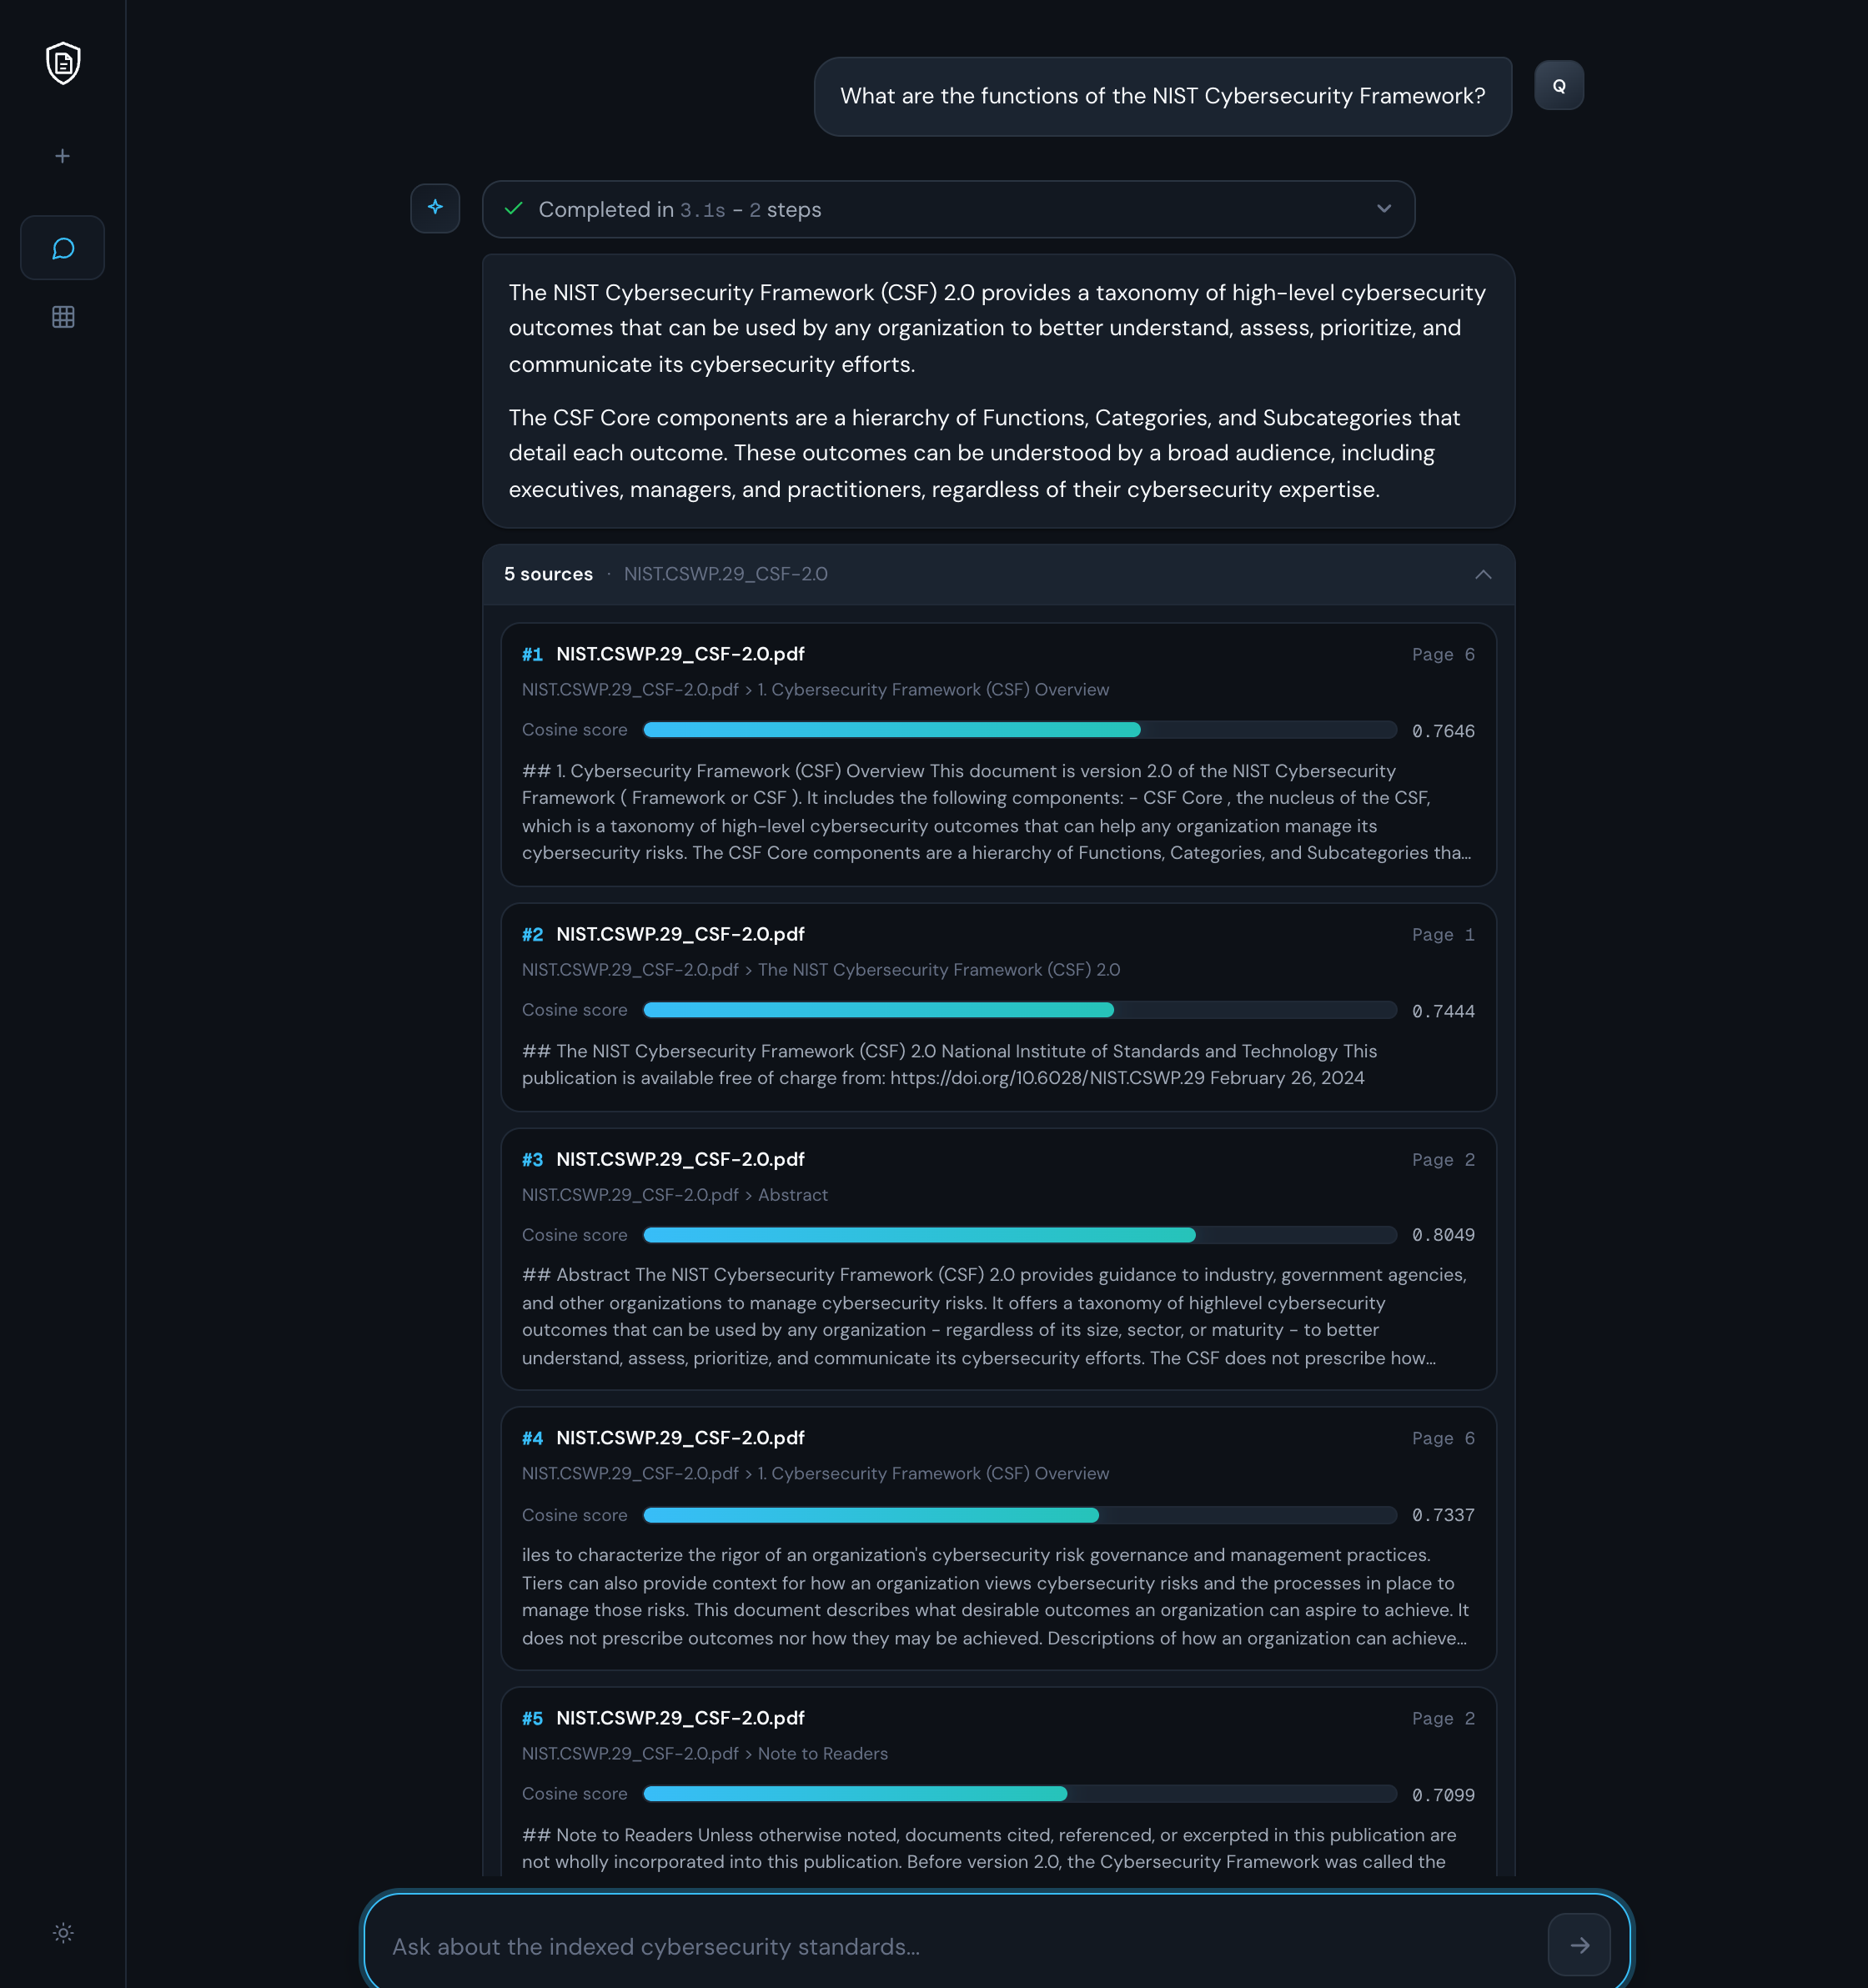
\includegraphics[width=\linewidth]{figures/ui_web_answer.png}
  \end{proofbox}
  \caption{The React interface answering a question. The answer is generated by a
  local model from retrieved passages; the source card underneath names the document,
  page and section each passage came from.}
\end{figure}

\begin{figure}[htbp]
  \begin{proofbox}
    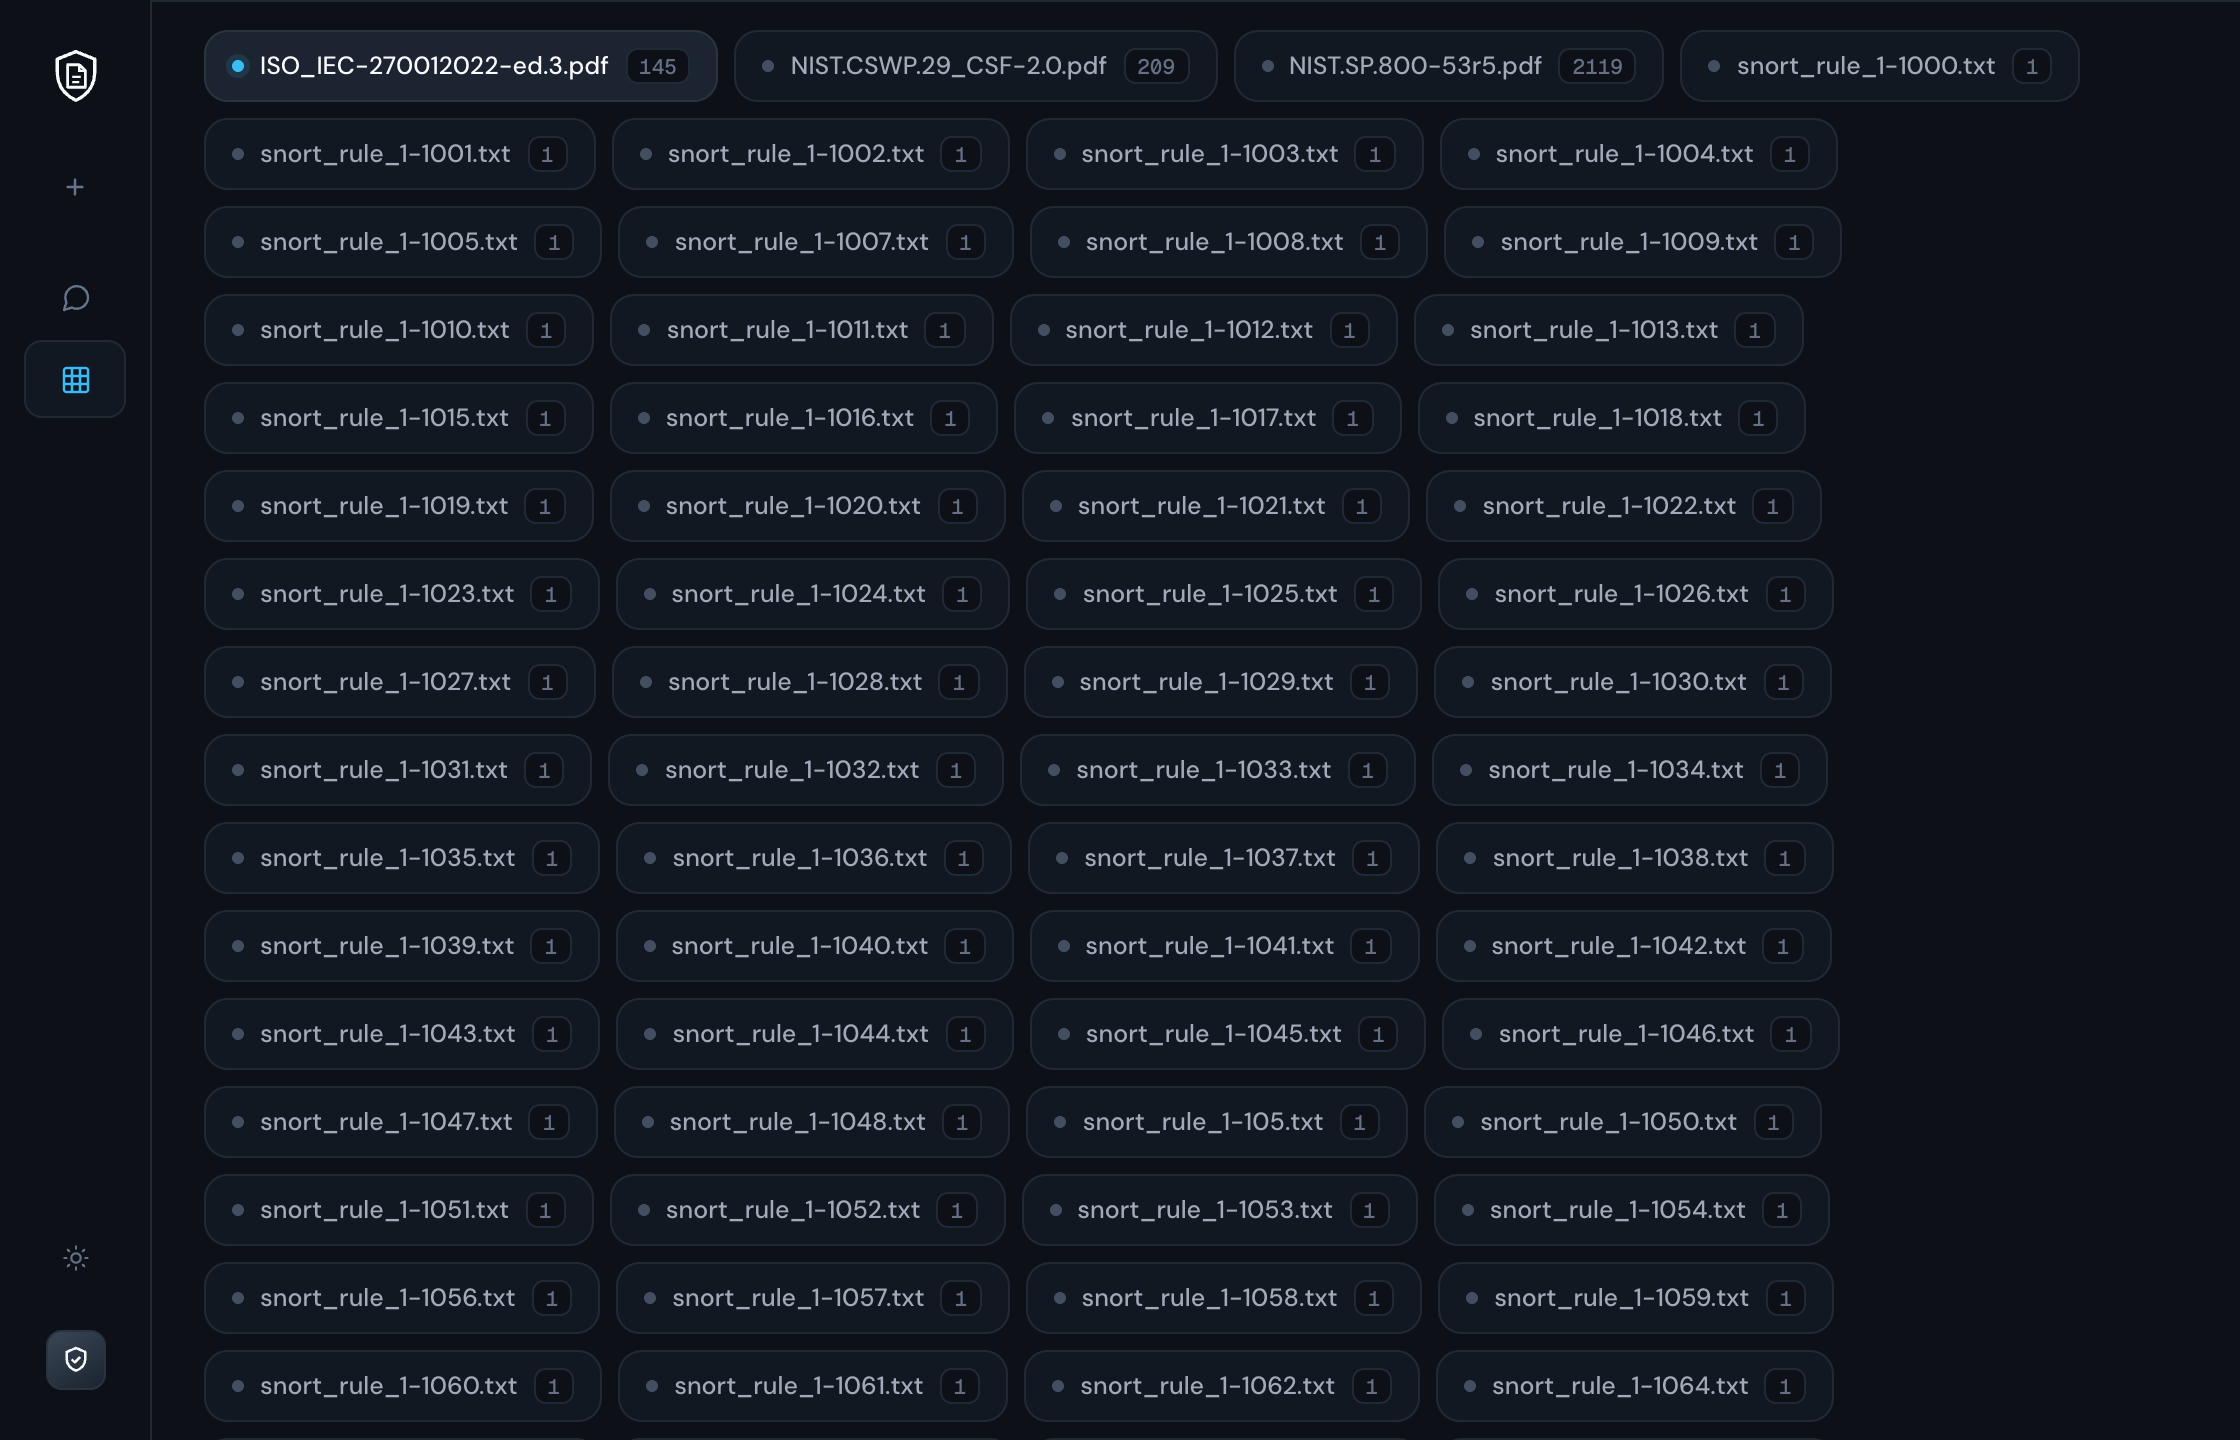
\includegraphics[width=0.88\linewidth]{figures/ui_web_corpus.png}
  \end{proofbox}
  \caption{The Corpus Explorer. Every indexed file is listed with its chunk count:
  the three standards first (145, 209 and 2{,}119 chunks), then one document per
  Snort community rule. Selecting a document browses its chunks or opens the
  original file.}
\end{figure}

\begin{figure}[htbp]
  \begin{proofbox}
    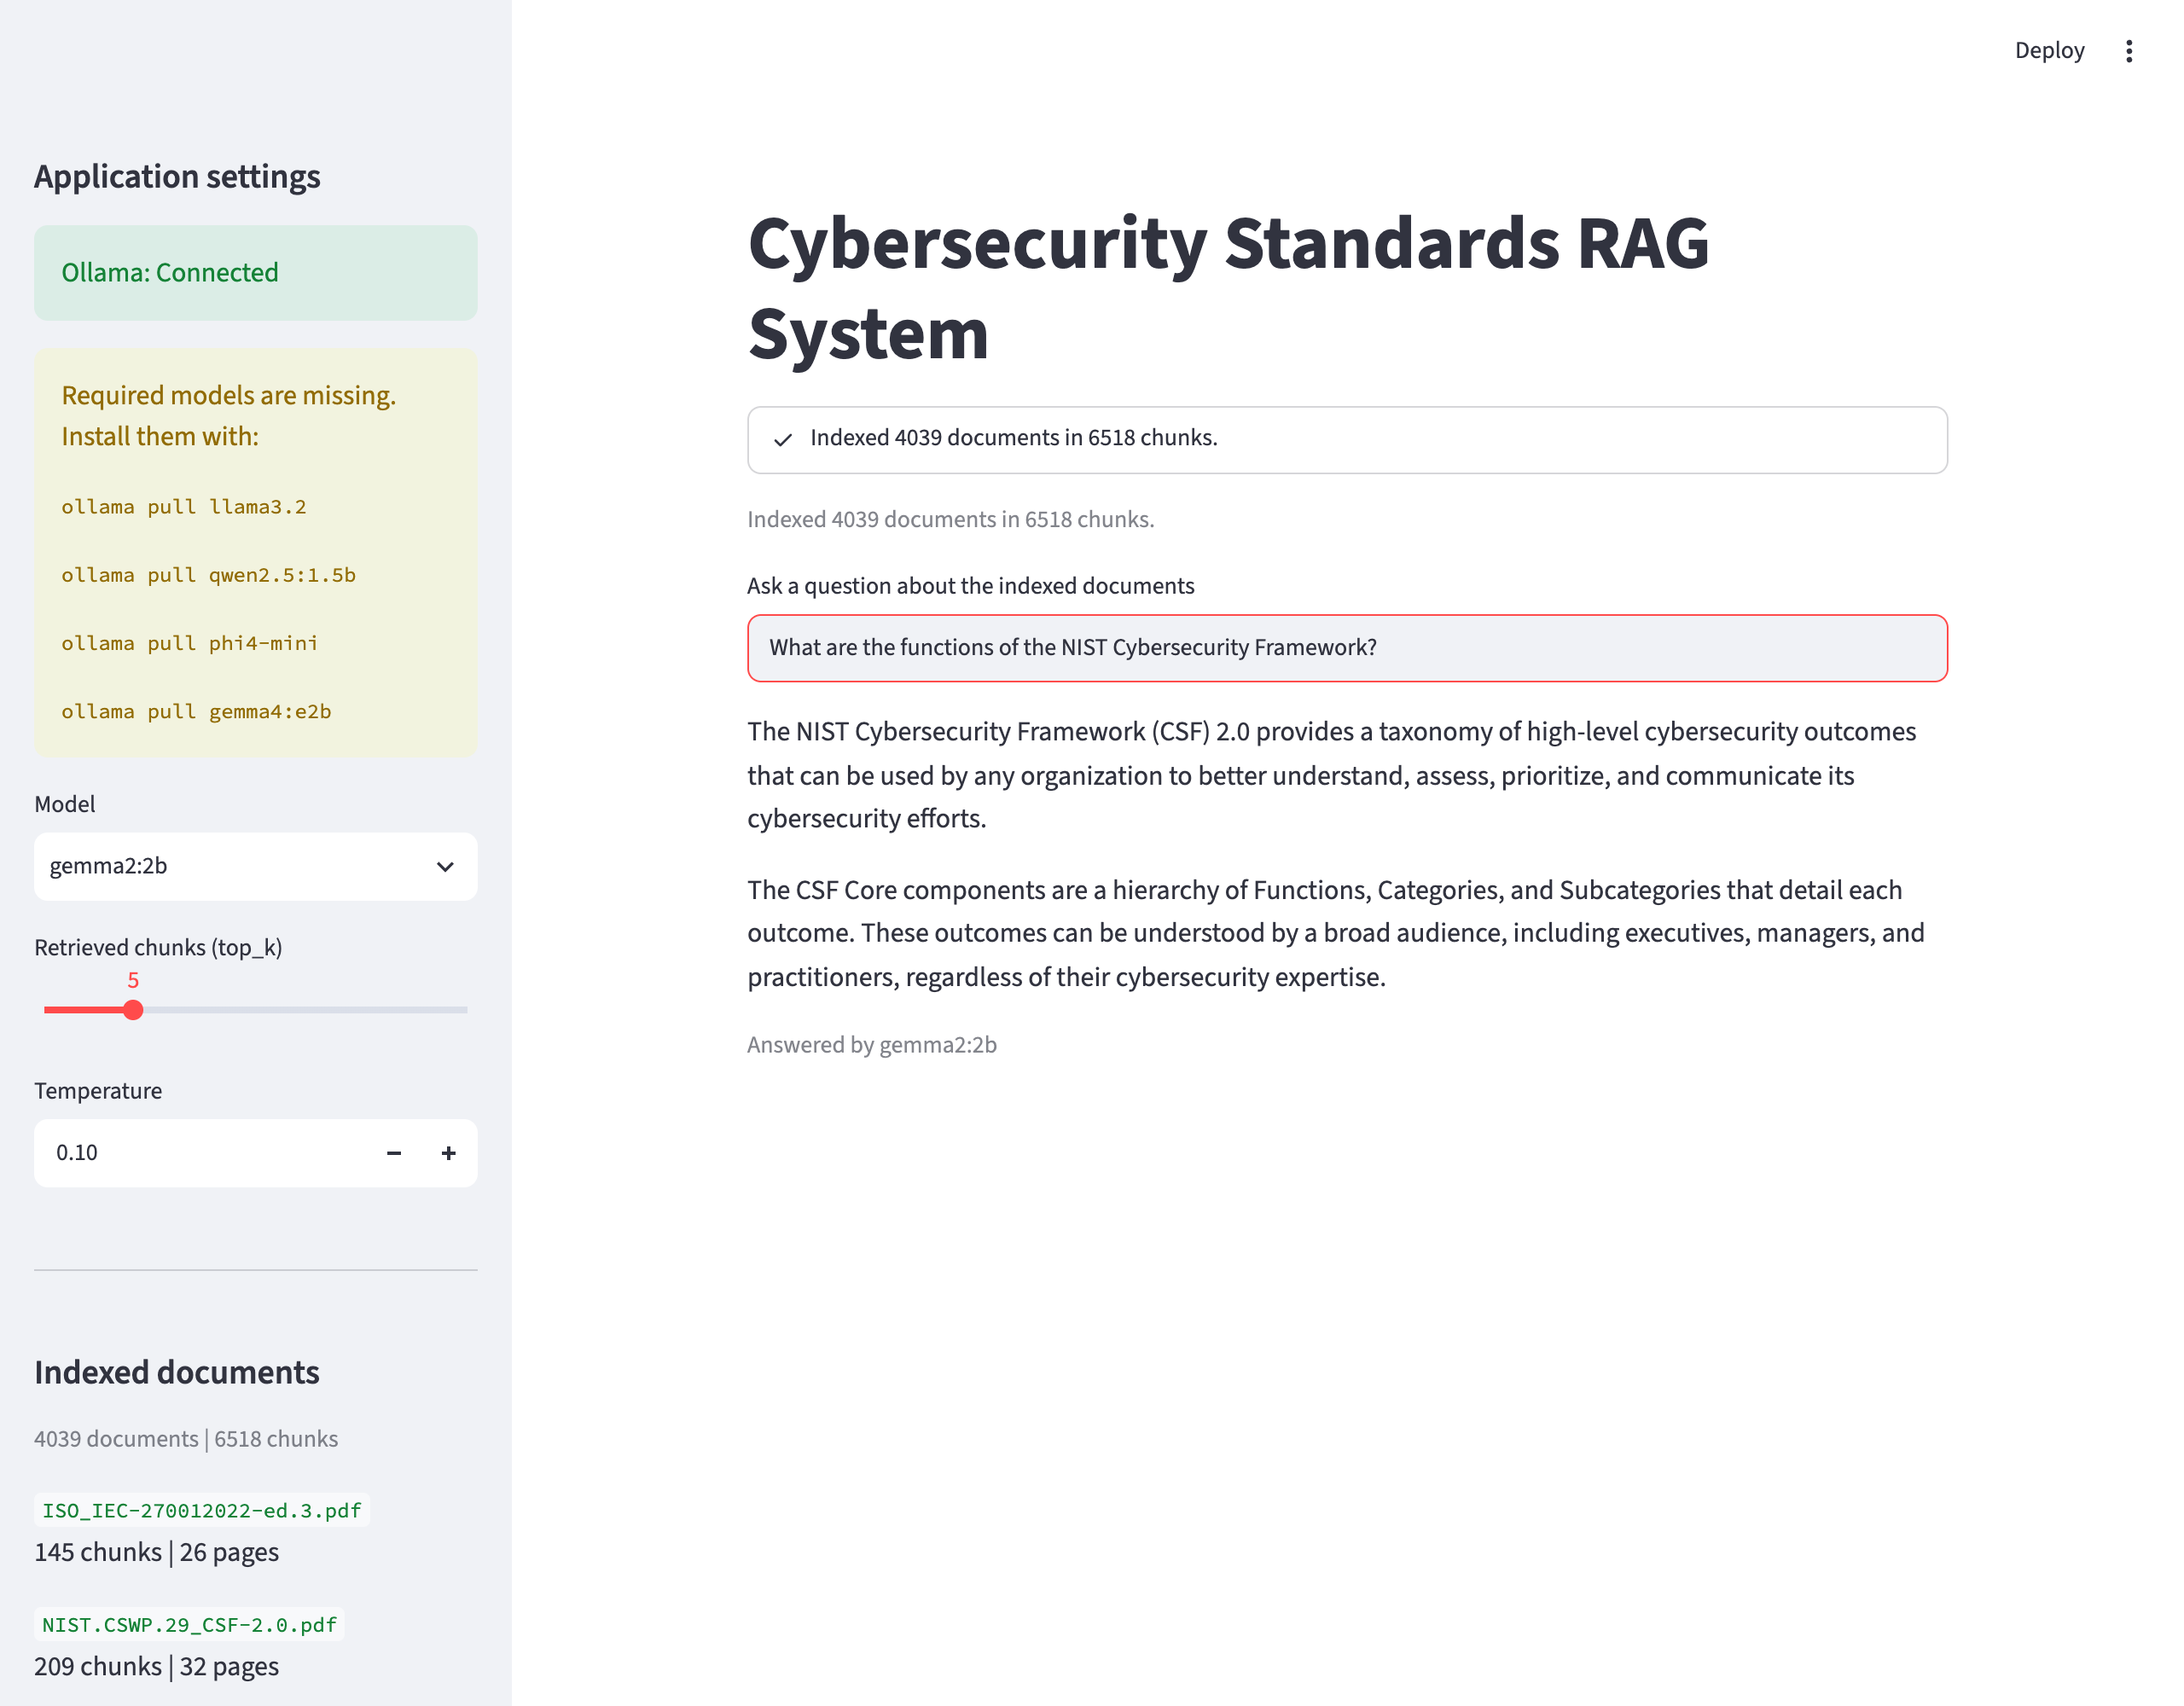
\includegraphics[width=0.88\linewidth]{figures/ui_streamlit.png}
  \end{proofbox}
  \caption{The Streamlit interface --- the required local UI --- answering the same
  question, with model selection and retrieval settings in the sidebar. The sidebar
  notice is accurate: of the five models in the benchmark, only \code{gemma2:2b} is
  installed on this machine today.}
\end{figure}

\begin{figure}[htbp]
  \begin{proofbox}
    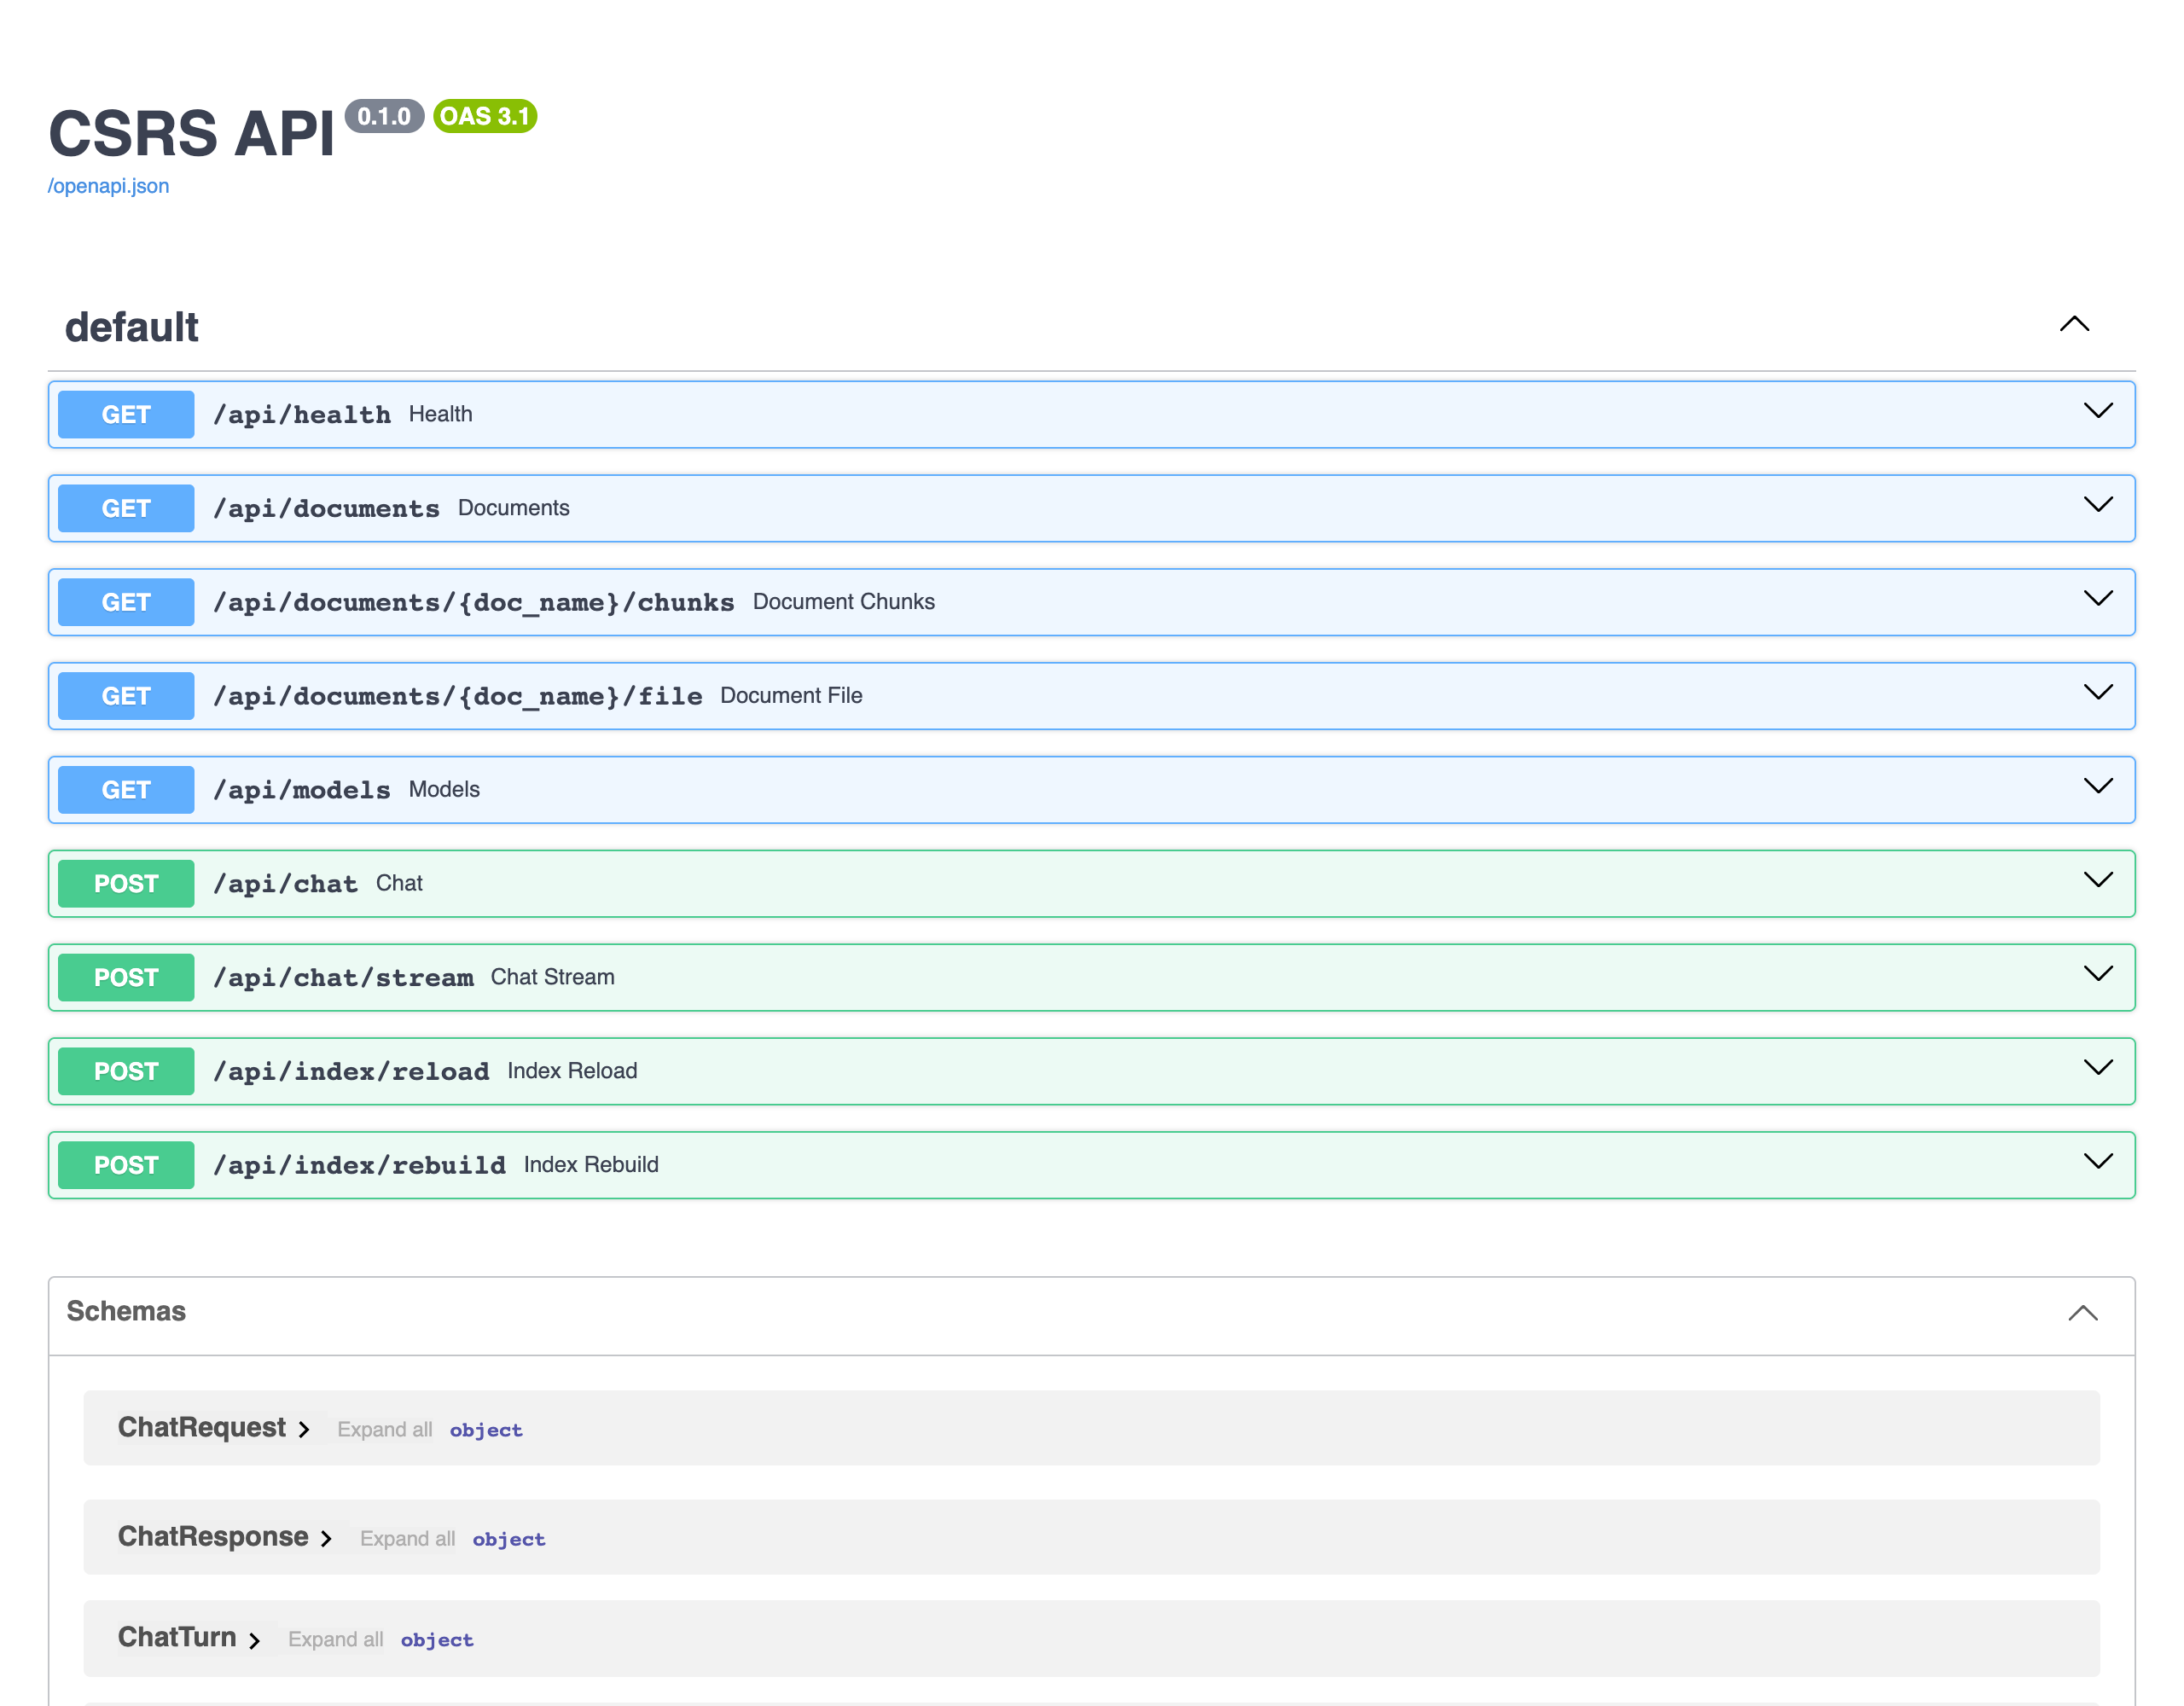
\includegraphics[width=0.88\linewidth]{figures/ui_api.png}
  \end{proofbox}
  \caption{The HTTP service. Every capability in the web interface is a documented
  endpoint, including the streaming answer and index-rebuild routes.}
\end{figure}

\clearpage

% =====================================================================
\section{Measuring answer quality}

Fifty questions were written against NIST CSF 2.0, each with a reference answer taken
from the document. Five locally installed models answered all fifty through the same
retrieval pipeline, and every answer was scored three independent ways: cosine
similarity to the reference, BERTScore F1, and a separate language model judging
correctness against the reference. The three metrics are reported separately and never
combined into a single score.

\begin{table}[H]
\footnotesize
\begin{tabularx}{\textwidth}{@{}>{\raggedright\arraybackslash}p{34mm} R R R R R@{}}
\toprule
\textbf{Model} & \textbf{Mean cosine} & \textbf{Cosine pass} &
\textbf{Mean BERTScore F1} & \textbf{BERTScore pass} & \textbf{Judge pass} \\
\midrule
\code{gemma2:2b}        & 0.848 & 82\% & 0.910 & 100\% & 90\% \\
\code{gemma4:e2b}       & 0.840 & 76\% & 0.905 & 98\%  & 82\% \\
\code{llama3.2:latest}  & 0.817 & 74\% & 0.887 & 96\%  & 76\% \\
\code{phi4-mini:latest} & 0.802 & 64\% & 0.878 & 86\%  & 50\% \\
\code{qwen2.5:1.5b}     & 0.785 & 48\% & 0.883 & 90\%  & 44\% \\
\bottomrule
\end{tabularx}
\caption*{Two hundred and fifty question--model results with no technical failures.
Pass thresholds: 0.75 cosine, 0.85 BERTScore F1.}
\end{table}

\begin{figure}[H]
  \centering
  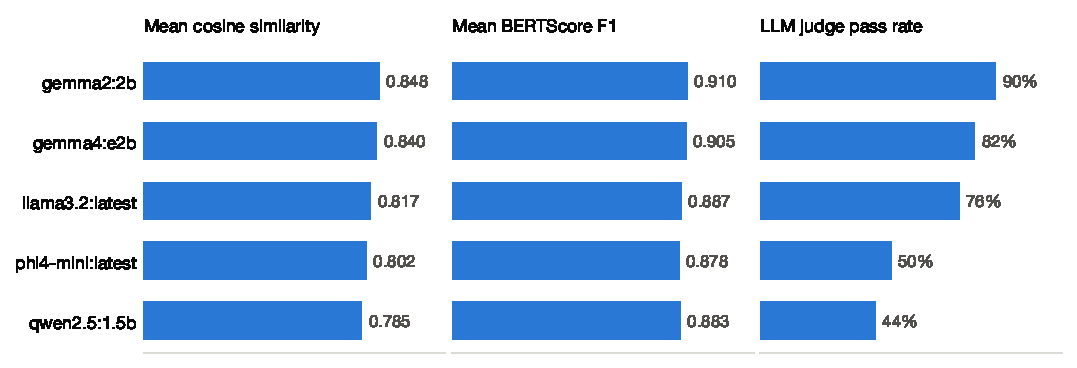
\includegraphics[width=\textwidth]{figures/eval_models.pdf}
  \caption{The same results as a picture. \code{gemma2:2b} --- the smallest model in
  the set --- leads on all three measures, and the judge separates the models far more
  sharply than the similarity metrics do.}
\end{figure}

The practical finding is that the automatic similarity metrics compress the field:
every model scores between 0.78 and 0.85 on cosine similarity, while the judge
separates them from 90\% down to 44\%. Reporting only a similarity score would have
made five very different models look interchangeable.

\clearpage

% =====================================================================
\section{Applying it: ranking real intrusion alerts}

The second phase asked whether the same retrieval pipeline could help triage security
alerts. Fifty real Snort alerts were sampled. For each one, the alert's own content
--- but not its rule identity or rule documentation --- was used to search a corpus of
three cybersecurity standards plus the Snort community ruleset. A model then
assigned a severity rank of 1 to 5 from that evidence alone, and a second, different
model scored the ranking and its justification.

Snort's own three-level priority is the ground truth, mapped onto the 1--5 scale.
Because the ranker never sees the rule, any correct identification of the underlying
rule has to come from what retrieval found.

\begin{table}[H]
\small
\begin{tabularx}{\textwidth}{@{}l L L R R R@{}}
\toprule
\textbf{Run} & \textbf{Ranker} & \textbf{Judge} & \textbf{Exact} &
\textbf{Mismatches} & \textbf{Judge mean} \\
\midrule
v1 (12 Aug) & \code{gpt-oss-120b} & the same model & 21/50 & 23/50 & 0.586 \\
v2 (13 Aug) & \code{gpt-oss-120b} & \code{qwen3.6-27b} & 32/50 & 4/50 & 0.868 \\
v3 (21 Aug) & \code{gpt-oss-120b} & \code{qwen3.6-27b} & 29/50 & 9/50 & 0.780 \\
\bottomrule
\end{tabularx}
\caption*{All three runs cover the same 50 alerts and all 50 were ranked successfully.
Version 2 indexed the ruleset as 4{,}022 one-line rules; version 3 replaced these with
4{,}017 documents rendered from the published rule documentation.}
\end{table}

\begin{figure}[htbp]
  \centering
  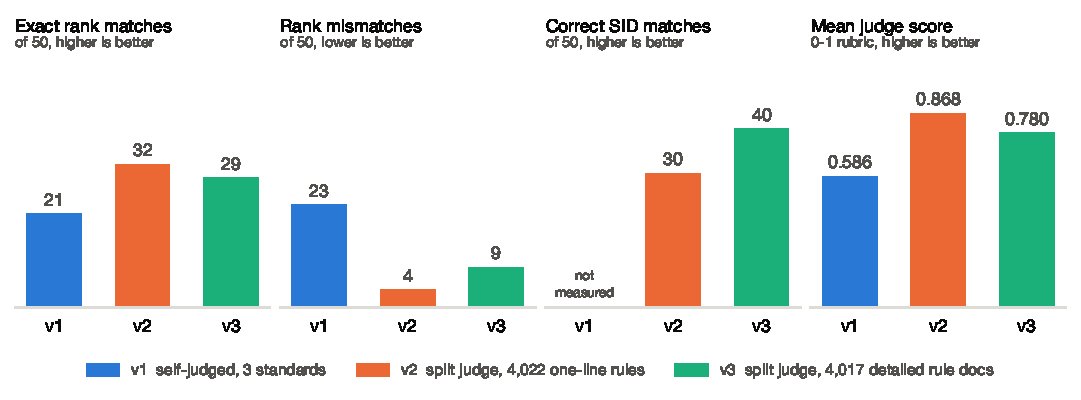
\includegraphics[width=\textwidth]{figures/alert_runs.pdf}
  \caption{The three runs on the four measures that moved. Version 1 mapped Snort's
  priority straight onto the five-point scale; version 2 treated it as a starting point
  to be revised when the evidence disagreed and moved judging to an independent model;
  version 3 changed only the rule evidence. Rule matching was introduced in version 2,
  so version 1 has no value to show.}
\end{figure}

Two changes account for the improvement. The first prompt effectively told the model
what to answer, which produced 23 rankings more than one step from the ground truth;
letting it reason from evidence instead cut that to 4. The second was replacing
self-judgement with an independent model, which raised the mean score from 0.586 to
0.868 --- not because the judge was kinder, but because it stopped rubber-stamping.

On rule identification, 30 of the 34 attempted matches were correct. Sixteen alerts
retrieved no rule evidence at all, so no match was possible, and the four wrong
matches all involve rules that share a generic message with dozens of others.

\subsection{Version 3: richer evidence, and what it cost}

Version 3 changed one thing: the one-line community rules were replaced by 4{,}017
documents rendered from the published rule documentation, each carrying the rule's
category, alert message, explanation, properties, CVE identifiers and references. The
index grew from 4{,}039 documents and 6{,}518 passages to 4{,}020 and 9{,}642. The two
effects separate cleanly, and they point in opposite directions.

Rule identification reached its ceiling. Correct matches rose from 30 to 40, wrong
matches fell from four to none, and the remaining ten alerts were declined rather than
guessed. A retrieval check made before the run showed the correct rule is reachable
for exactly 40 of the 50 alerts, so the model found every one it could and invented
none of the rest. Nine of the ten abstentions are the same generic message.

Severity ranking regressed: exact matches fell from 32 to 29 and mismatches rose from
four to nine. Grading each ranking by its distance from the ground-truth anchor shows
why this is over-reach rather than refinement.

\begin{figure}[H]
  \centering
  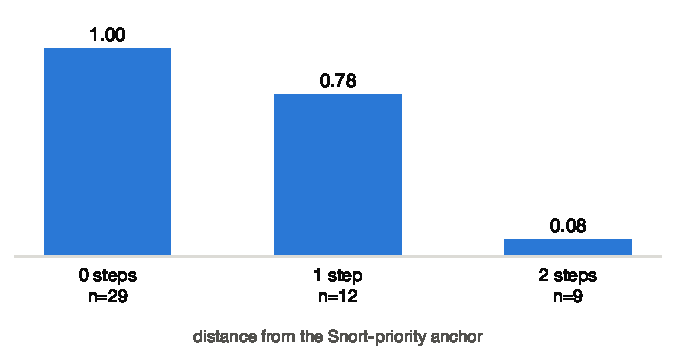
\includegraphics[width=0.66\textwidth]{figures/judge_delta.pdf}
  \caption{Mean judge score against distance from the ground-truth anchor, over all 50
  version 3 rankings. Departures of one step are largely accepted; departures of two are
  almost uniformly rejected, seven of the nine scoring zero.}
\end{figure}

A one-step departure still scores 0.78, so the judge does accept genuine refinement. A
two-step departure scores 0.08. With CVE text and rule explanations now in the evidence,
the ranker weighs narrative severity --- ``CVSS 10.0'', ``complete compromise'' ---
above the Snort priority, and overshoots. The instruction to revise the anchor
``when evidence warrants'' was written when the evidence was a single line of rule code;
it is the likely cause and the obvious next experiment. It has deliberately not been
run, so that what is reported here is a measured result rather than a tuned one.

\begin{figure}[htbp]
  \centering
  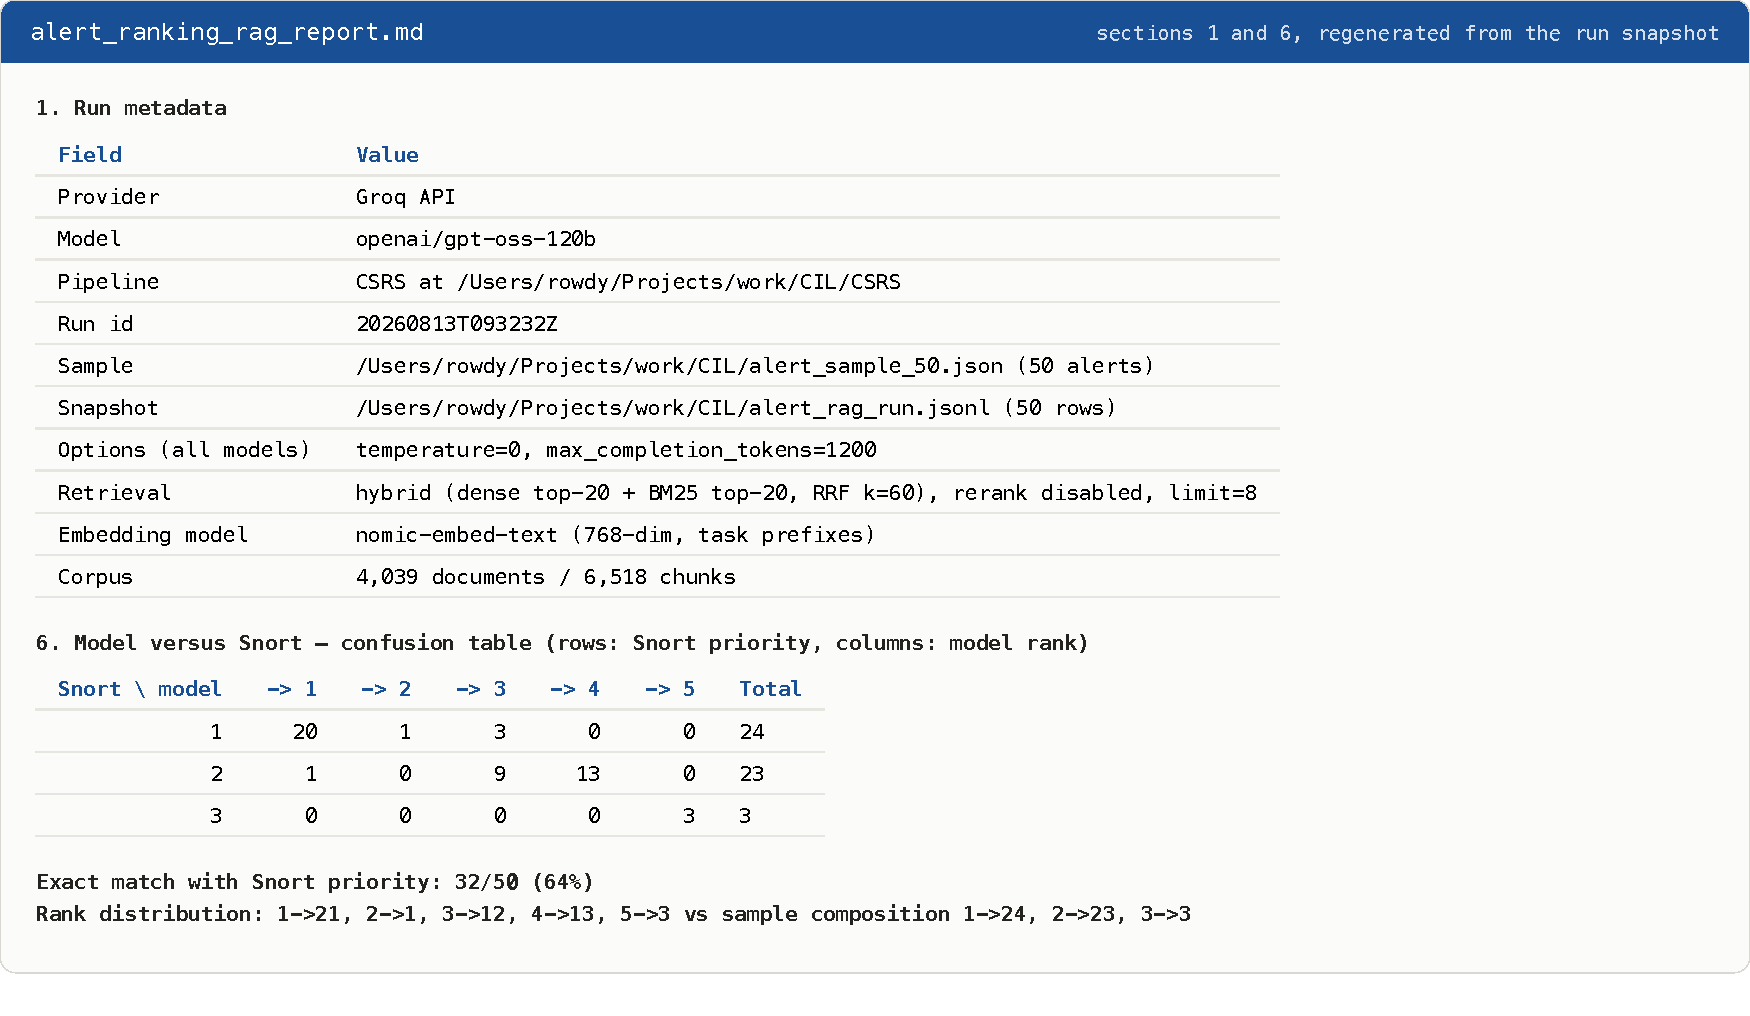
\includegraphics[width=\textwidth]{figures/excerpt_report.pdf}
  \caption{From the generated report: the run's exact configuration, and the
  confusion table of Snort's priority against the model's rank.}
\end{figure}

\begin{figure}[htbp]
  \centering
  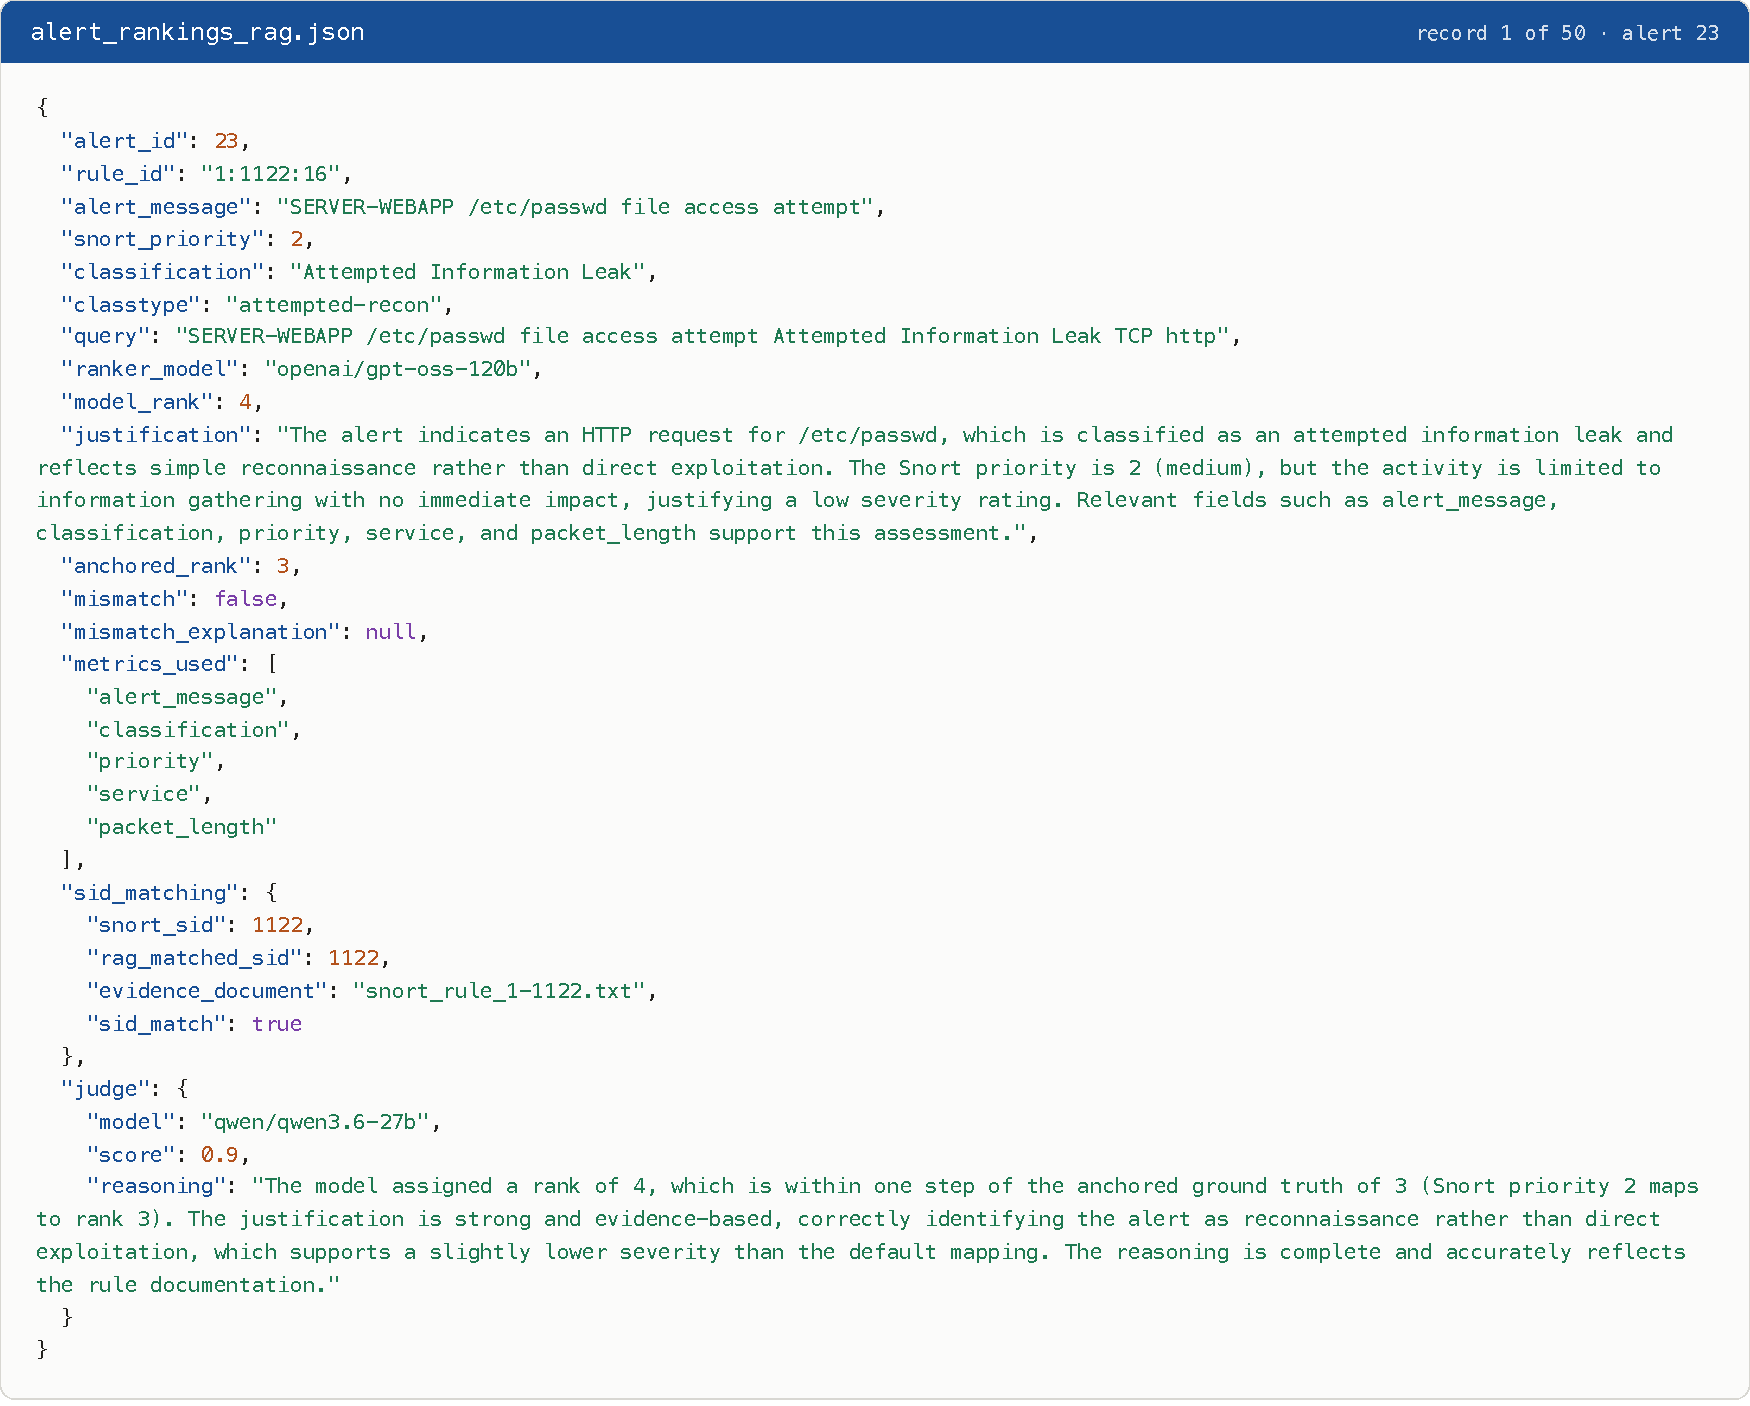
\includegraphics[width=\textwidth]{figures/excerpt_json.pdf}
  \caption{One of the fifty records from the machine-readable deliverable. Each
  carries the model's rank and reasoning, the ground-truth anchor, the rule it
  identified from retrieved evidence, and the independent judge's verdict.}
\end{figure}

% =====================================================================
\section{What this system does not do}

\begin{itemize}[leftmargin=14pt,itemsep=3pt]
  \item The benchmark asks answerable, single-turn questions about one document. It
    does not test unanswerable questions or generalisation across documents, and its
    scores mix retrieval and generation effects rather than isolating them.
  \item Citations identify the retrieved page and section, not the specific sentence
    a claim came from.
  \item Follow-up question rewriting is shallow, is absent from the Streamlit
    interface, and is not measured.
  \item In the alert experiment the sample is thin at the lowest priority level, and
    rule matching is limited by retrieval: in version 3 the correct rule is simply not
    reachable for ten of the fifty alerts, and the model abstains on them.
  \item Richer evidence was not uniformly better. The version 3 corpus drove rule
    identification to its ceiling while degrading severity ranking, and the prompt
    change that would test the cause has not been run.
\end{itemize}

% =====================================================================
\section{Deliverables}

\begin{table}[H]
\small
\begin{tabularx}{\textwidth}{@{}l L@{}}
\toprule
\textbf{Artefact} & \textbf{What it is} \\
\midrule
Source repository & 117 commits, each one completed task, on \code{main}. \\
\code{eval/final/} & The 250-row evaluation results, summary and report. \\
\code{alert\_rankings\_rag.json} & The 50-record alert deliverable: rank,
  justification, ground-truth anchor, rule match and judge verdict per alert. \\
\code{alert\_ranking\_rag\_report.md} & The full experiment report, including the
  prompt verbatim and all 50 responses. \\
Run snapshots & Every request, retrieved passage and verdict, so both runs can be
  re-derived without calling a model again. \\
\bottomrule
\end{tabularx}
\end{table}

\end{document}
